\section{Exploring Thread Interleaving Space}
\label{s:design}

In this section, we describe our approach to effectively achieve
\textbf{Design goal 1} and \textbf{2}.
%
We first explain the key idea of our approach~(\autoref{ss:overview}). 
At first, we illustrate our concurrency
coverage metric to express combinatorial interleavings 
(\textbf{Design goal 1})~(\autoref{ss:coverage}) and the instruction scheduling mechanism
to quickly saturate the coverage metric (\textbf{Design goal 2})~(\autoref{ss:scheduler}).
%While this section focuses only on how to explore the search space of
%thread interleaving with a given multi-thread input, the whole design
%of \sys will be explained later in \autoref{s:impl}.


\subsection{Key Idea: Segmentizing thread interleaving}
\label{ss:overview}

\begin{table}[t]
  \centering
  \resizebox{0.95\linewidth}{!}{
  \begin{tabular}{l | r r r r r | r}
    \toprule
    \textbf{\# of acc.} & \textbf{1 acc.} & \textbf{2 acc.} & \textbf{3 acc.} & \textbf{4 acc.} & \textbf{>4 acc.} & \textbf{Total}\\
    \midrule
    \# of bugs & 7 & 25 & 53 & 12 & 8 & 105 \\
    \bottomrule
  \end{tabular}
}

%%% Local Variables:
%%% mode: latex
%%% TeX-master: "../p"
%%% End:

  \caption{Statistics provided by Shan Lu
    \etal~\cite{learningfrommistakes}, stating the number of
    concurrency bugs according to the number of memory accesses
    involved in the manifestation of a concurrency bug.}
  \label{table:learningfrommistakes}
\end{table}

When fuzzing concurrency bugs with a coverage metric, the fundamental challenge is its large search space because
the combinations of thread interleavings increase the 
the search space exponentially. Therefore, this work seek to 
strike the balance
in the trade-off between bug-finding capability and search 
complexity. Observed by a previous study~\cite{learningfrommistakes}
as shown in \autoref{table:learningfrommistakes}\yj{Do we need the table?}, 92.4\% (97 out of
105) of concurrency bugs manifest when a bug-finding system 
monitors instruction execution orders including \textit{at most} 
four memory accesses referring to the same object\yj{the same address?}.
All other memory
accesses beyond four accesses and their execution orders do not
meaningfully affect manifestation of a concurrency bug. 
The observation also is applied to the example of \autoref{fig:cve-2017-17712}. The uninitialized access bug is triggered by 
the execution order of three
memory accesses (\eg, \texttt{A2}, \texttt{A4} and \texttt{B1}), while
others (\eg, \texttt{A6} and \texttt{B2}) are irrelevant to manifest the
concurrency bug.


\PP{Segmentizing thread interleaving}
To reduce the search complexity, we take the classical wisdom of problem decomposition where 
complexity of a problem exponentially decreases as the problem size decreases.
Our key strategy is \textit{decomposing} the search space into 
small sub-spaces. We call a sub-space \textit{interleaving segment}.
Each interleaving segment consists of instructions accessing 
the same memory addresses (i.e., conflicting instructions).
When constructing a interleaving segment, following the observation, 
we confine the size of a interleaving segment 
to contain interleaved instructions including at most four memory accesses,
which makes the problem of defining a coverage metric tractable while maintaining a strong bug-finding capability.

\PP{Building segments}
%
In particular, once executing threads concurrently, we firstly model
the thread interleaving as a totally-ordered instruction sequence.
%
And then, we group a small number of instructions (\eg, four
instructions) and their interleaving orders as an interleaving segment.


\begin{figure*}[t]
  \centering
  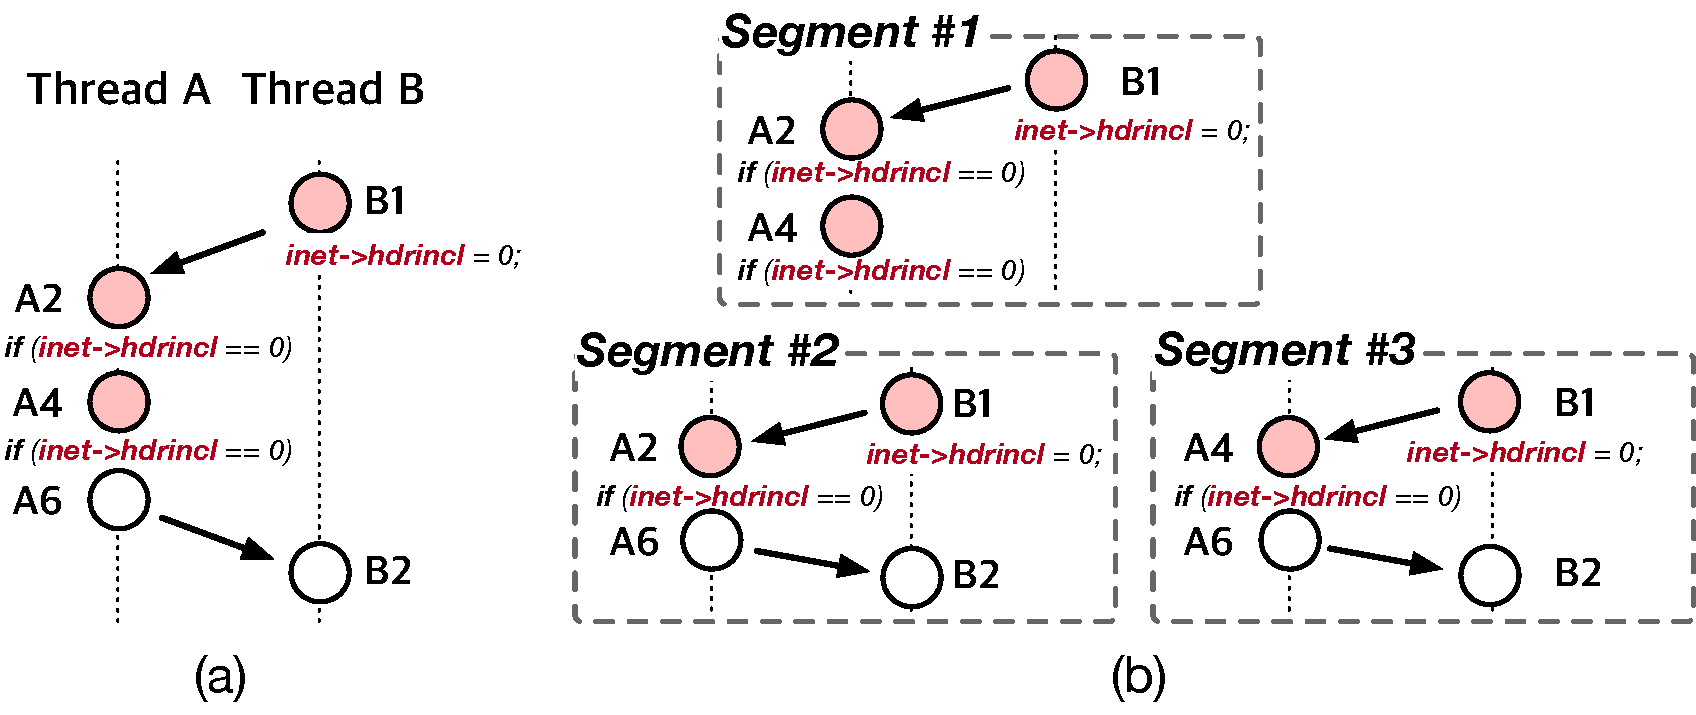
\includegraphics[width=0.9\linewidth]{fig/intuition.pdf}
  \caption{(a) A thread interleaving example of
    \autoref{fig:cve-2017-17712} that does not cause the concurrency
    bug, (b) instruction pairs that access the same memory object,
    and (c) instruction segments composed of two instruction pairs.
    Note that we intentionally omit instructions that do not access
    globally-visible memory objects.}
  \label{fig:keyidea}
\end{figure*}
%
\autoref{fig:keyidea} visualizes our key idea.
%
Let us assume we execute the two system calls in
\autoref{fig:cve-2017-17712} concurrently.
%
\autoref{fig:keyidea}-(a) represents the thread interleaving of the
execution, where the uninitialized access bug does not manifest
because \texttt{B1} is executed after \texttt{A4} (\ie,
$(\texttt{A2} \Rightarrow \texttt{B1}) \wedge (\texttt{B1} \Rightarrow
\texttt{A4})$ is not satisfied).
%
In order to track interleaving orders of a small number (\eg, four) of
instructions, we decompose the thread interleaving into several
interleaving segments as described in \autoref{fig:keyidea}-(b).
%
In these interleaving segments, \texttt{Segment \#1} contains three
memory access operations (\ie, \texttt{A2}, \texttt{A4}, and
\texttt{B1}), and describes interleaving orders such that \texttt{B1}
is executed after \texttt{A2} and \texttt{A4}.
%
Similarly, \texttt{Segment \#2} and \texttt{Segment \#3} describes
interleaving orders of four memory access operations, (\texttt{A2},
\texttt{B1}, \texttt{B2}, \texttt{A6}) and (\texttt{A4}, \texttt{B1},
\texttt{B2}, \texttt{A6}) respectively.
%

% With these interleaving segments, the fuzzer can be noticed that
% interleaving orders represented by these interelaving segments
% unlikley cause a concurrency bug.
% %
% Therefore, it is adequate for the fuzzer to search for unexplored
% interleaving segments (\eg, one that represents
% $(\texttt{A2} \Rightarrow \texttt{B1}) \wedge (\texttt{B1} \Rightarrow
% \texttt{A4})$) to maximize the chance of discovering concurrency bugs.


%
It is worth noting that interleaving segments can be overlapped; in
this example, \texttt{Segment \#1} and \texttt{Segment \#3} are
overlapped over an interleaving order
$\texttt{A4} \Rightarrow \texttt{B1}$.




\PP{Benefits of segmentizing thread interleaving}
%
Segmentizing thread interleaving provides two remarkable benefits to
the fuzzer as follows.



First, tracking interleaving segments is a befitting choice to
determine if any interesting thread interleaving remains untested.
%
As mentioned above, most concurrency bugs manifest depending only on
the execution order of four memory access operations. If the fuzzer
explores all interleaving segments with size of at most four, it is
unlikely that the fuzzer misses a concurrency bugs.
%
Accordingly, \textit{interleaving segments can be act as an
  interleaving coverage metric that allows a fuzzer to satisfy
  \textbf{R1}}.
  

In the example of \autoref{fig:cve-2017-17712}, \dr{TODO: conect to the exapmle}




Second, explored interleaving segments can be exploited to
\textit{direct} the fuzzer about what thread interleaving needs to be
explored in future.
%
\autoref{fig:hint} demonstrates how explored interleaving segments
can be helpful for future iterations.
%
As illustrated in \autoref{fig:hint}, the fuzzer can derive
\textit{unexplored} \texttt{Segment \#1*} by changing the execution
order of \texttt{A4} and \texttt{B4} in \textit{explored}
\texttt{Segment \#1}.
%
Since \texttt{Segment \#1*} satisfies
$(\texttt{A2} \Rightarrow \texttt{B1}) \wedge (\texttt{B1} \Rightarrow
\texttt{A4})$, the fuzzer can discover the uninitialized access bug if
it executes thread interleaving containing \texttt{Segment \#1*}.
%
In addition, the fuzzer can explore multiple interleaving segments at
a time.
%
Besides \texttt{Segment \#1*}, \texttt{Segment \#3*} can also be
derived from \texttt{Segment \#3}.
%
Interestingly, \texttt{Segment \#1*} and \texttt{Segment \#3*} can be
used to compose a new thread interleaving.
%
By executing a thread interleaving including the two derived
interleaving segments, the fuzzer is able to quickly test a number of
interleaving segments.
%
In this way, \textit{our proposed scheduler mechanism is designed to
  quickly explore unexplored interleaving segments, and to satisfy
  \textbf{R2}}.
%
\begin{figure}[t]
  \centering
  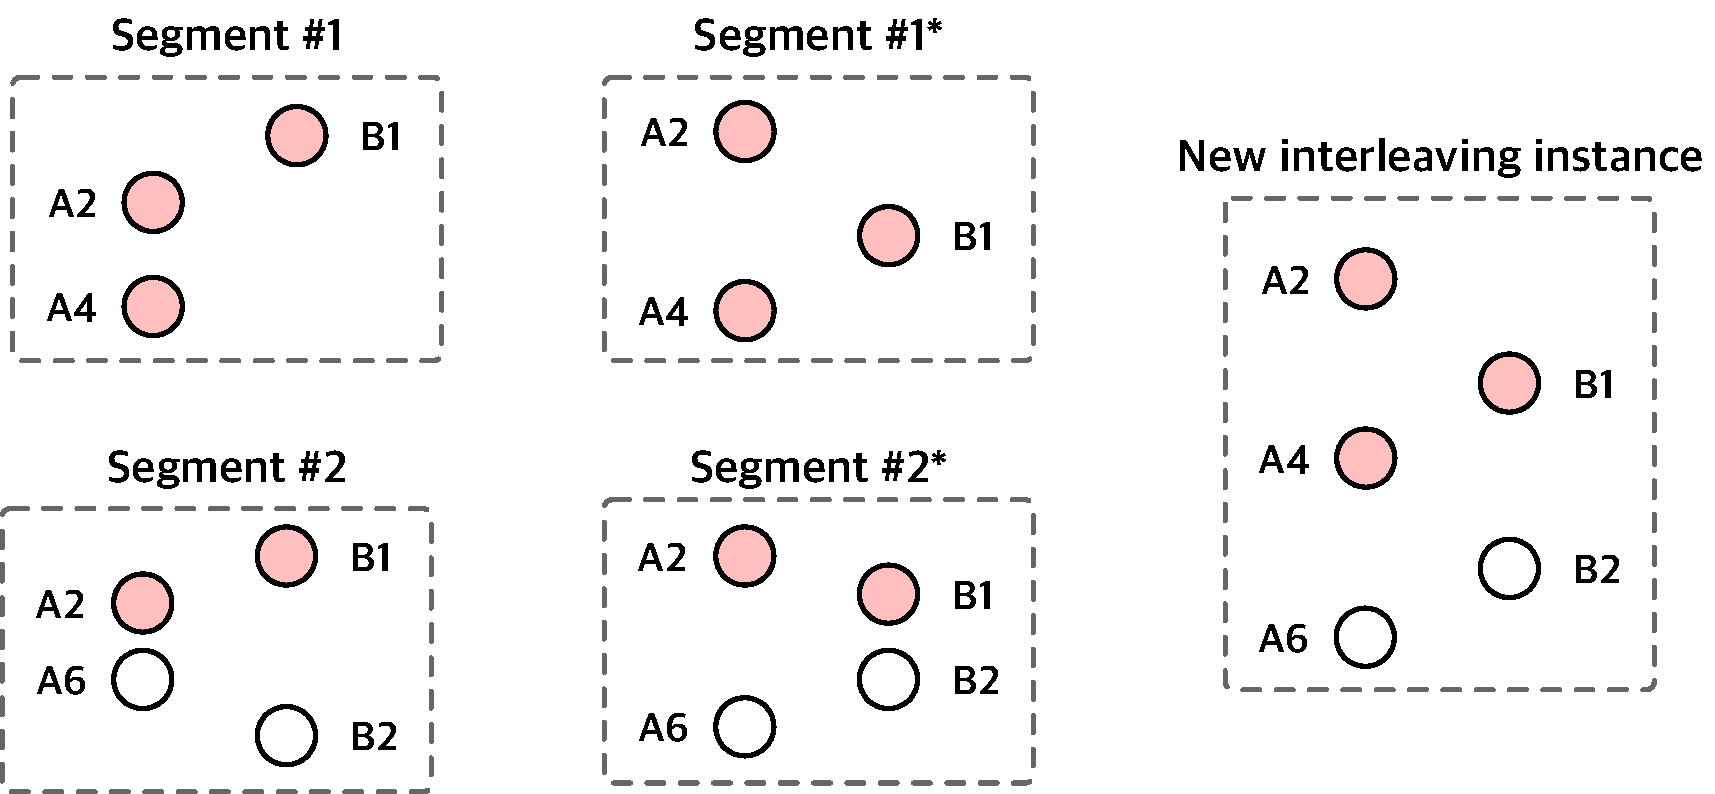
\includegraphics[width=0.9\linewidth]{fig/hint.pdf}
  \caption{\texttt{Segment \#1} and \texttt{Segment \#3} are explored
    interleaving segments in \autoref{fig:keyidea}.
    %
    From these two interleaving segments, our approach derives other
    interleaving segments \texttt{Segment \#1*} and \texttt{\#3*}, and
    schedules instructions to test the derived interleaving segments
    at the same time.}
  \label{fig:hint}
\end{figure}
%



\subsection{Interleaving Segment Coverage}
\label{ss:coverage}

\newcommand{\mutable}{mutable edge\xspace}
\newcommand{\mutables}{mutable edges\xspace}
\newcommand{\immutable}{immutable edge\xspace}
\newcommand{\immutables}{immutable edges\xspace}
\newcommand{\intcov}{interleaving segment coverage\xspace}
\newcommand{\Intcov}{Interleaving segment coverage\xspace}


Using a set of interleaving segments, we propose a novel concurrency coverage metric called \textit{\intcov}.
\Intcov is designed to track interleaving orders
within an interleaving segment and used for guiding a fuzzer to  
efficiently search possible instruction interleavings.
If \Intcov of a given input is saturated, 
a fuzzer can confidently conclude that the input unlikely causes a concurrency bug and proceed to the next input.

\PP{Graph representation of interleaved instructions}
As discussed, \Intcov contains multiple interleaved instructions, 
so \intcov cannot be presented as a single instruction interleaving 
(e.g., $I_x \rightarrow I_y$) used in the alias coverage used in KRace.
Instead, we represent each interleaving segment as a small directed acyclic
graph (DAG) called an interleaving segment graph (shortly, \textit{interleaving graph}), and \intcov is a collection of interleaving graphs.
%
In this graph, a vertex represents a memory-accessing instruction, 
and an edge represents an execution ordering between two memory-access instructions. 
Specifically, there are two types of edges, program-order edges and
interleaving-order edges.
%
A program-order edge indicates an execution order between two 
memory-accessing instruction in a single thread.
Whereas, an interleaving-order edge indicates the execution
order between two memory-access instructions that 1) access the same
shared data, 2) at least one of them is a write operation, and 3) are
executed by different threads.
\autoref{fig:interleavingsegmentgraph} illustrates how a interleaving 
graph is derived from a interleaving segment, \texttt{Segment \#1}.
This interleaving graph contains a program-order edge from \texttt{A2} to
\texttt{A4} representing ``\texttt{A2} is executed before \texttt{A4}
in thread~A''.
The interleaving graph contains two interleaving-order
edges, expressing execution orders of \texttt{A2} $\rightarrow$ \texttt{B1}
and \texttt{A4} $\rightarrow$ \texttt{B1}.
%It contains an interleaving-order edge from \texttt{A2} to
%\texttt{B1}, because 1) they access \texttt{inet->hdrincl}, 2)
%\texttt{B1} is a write operations, and 3) they are executed by
%different threads. Likewise, the segment graph also contains an
%interleaving-order edge from \texttt{A4} to \texttt{B1}.



\begin{figure}[t]
  \centering
  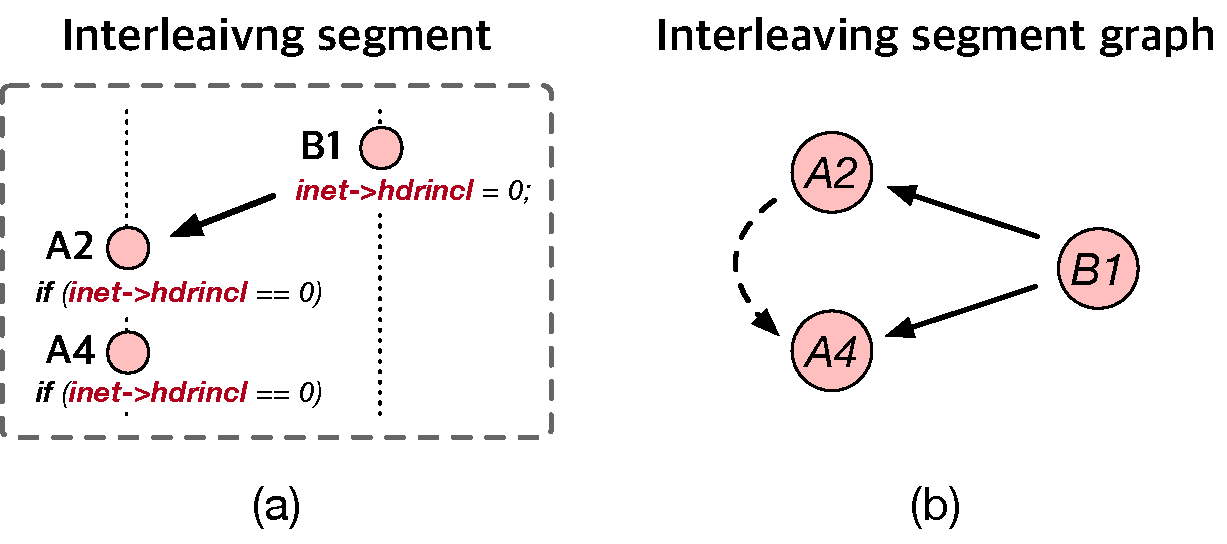
\includegraphics[width=0.9\linewidth]{fig/interleavingsegmentgraph.pdf}
  \caption{\texttt{Segment \#1} and its segment graph. A
    dotted arrow represents a program order, and solid arrows
    represent interleaving orders.}
  \label{fig:interleavingsegmentgraph}
\end{figure}

%It is worth noting that a segmentgraph has two properties. First, if
%a path exists from a vertex \texttt{X} to another vertex \texttt{Y}, a
%memory access operation corresponding to \texttt{X} is executed before
%a memory access operation corresponding to \texttt{Y}.
%%
%\dr{}
%This is because edges represent orderings that are a transitive
%relation.
%
%Second, \textit{all segment graph cannot contain a loop}.
%%
%If there is a loop exists, any vertex \texttt{Z} on the loop is
%executed before itself, which is contradictory.


%
% Let us represent a memory access operation $M$ as four tuples,
% $(tid, addr, op, timestamp)$ where $tid$ is the identity of a thread,
% $addr$ is the address of a memory location, $op$ is the type of the
% memory access operation (\ie, $store$ or $load$), and $timestamp$
% indicates the point of time when the memory access operation is taken.
% %
% $M(x)$ detnoes a field $x$ of $M$. For example, $M(tid)$ is a $tid$
% field of a memory access operation $M$.
% %
% Also let us suppose all memory access operations are totally
% ordered. \ie, there are no two memory access operations that have the
% same $timestamp$.

% For all pair of memory access operations $M_i$ and $M_j$, we define a
% scheduling constraint $SC$ as a tuple $(M_i, M_j)$ if
% $M_i(tid) \neq M_j(tid)$, $M_i(addr) = M_j(addr)$,
% $M_i(op) = store \vee M_j(op) = store$, and
% $M_i(timestamp) < M_j(timestamp)$.
% %
% Informally, $M_i$ and $M_j$ are conflicting memory acceess operations
% that are executed in other threads, and $M_i$ was taken place before
% $M_j$.
% %
% For two scheduling constraint $SC_1(M_{1i}, M_{1j})$ and
% $SC_2(M_{2i}, M_{2j})$, $SC_1 = SC_2$ if
% $(M_{1i} = M_{2i}) \wedge (M_{1j} = M_{2j})$.
% %
% Then, we define a scheduling constraint pair $SCPair = (SC_i, SC_j)$
% for two scheduling constraints if $i < j$, $SC_i \neq SC_j$.
% %
% Lastly, biconflict coverage of the concurrent job $BC\mbox{-}Cov$ is
% defined as a set of all scheduling constraint pairs,
% $\{SCPair_1, SCPair_2, ..., SCPair_n\}$, constructed from its memory
% access operation sequence.


\PP{Tracking interleaving segment coverage}
We track interleaving segment coverage \textit{offline}. While
executing a multi-thread input, a fuzzer collects memory-access
instructions annotated with timestamps. After the execution is
finished, the fuzzer collect segments and then builds interleaving 
graphs for each segment to compute \intcov for the given input.
In practice, \intcov contains a large number of interleaving graphs, 
whic consumes a large amount of memory even thought the size of graphs is 
small.
To reduce memory consumption, we hash each segment graph,
and interleaving segment coverage tracks a hash table of segment
graphs.
%
\dr{TODO: explain how to hash the graph}\yj{Fill this, I will edit later.}


% \dr{heuristic}
% %
% size 3 and 4
% %
% no containing a vertex that is not connected with interleaving order



\PP{Utilizing interleaving segment coverage}
Compared to the alias coverage, \intcov and the form of interleaving graph
express semantically richer information. \Intcov captures combinations 
of multiple memory-accessing instructions as a unit of an interleaving segment, which allows a fuzzer to explore the large search space more quickly than using alias coverage, which uses a single instruction interleaving. Intuitively, across two different runs, \intcov can precisely tell 
their differences in terms of at least two instruction interleavings, 
but the alias coverage can tell at least one\yj{DR, it this claim OK to you?}.
\Intcov provides guiding feedback to a fuzzer.
\Intcov guides the fuzzer to identify that there are possibly more useful instruction interleavings remain untested. So, the fuzzer spends
more computing power to explore more interesting (unseen) instruction interleavings from \intcov. We emphasize that our searching strategy is 
\textit{not random} unlike previous approaches~\yj{cites}.
We use\yj{transform? better word?} a newly found interleaving graph 
to direct the fuzzer to systematically explore 
the search space of instruction interleavings while minimizing
redundant and useless search trials. \autoref{ss:scheduler} 
discusses our search strategy.


\subsection{Coverage-directed Thread Scheduling Control}
\label{ss:scheduler}
%
One important role of segment graphs are to infer unexplored
interleaving segments that the fuzzer will search for in future
iterations.
%
In this subsection, we explain how we generate scheduling points in
order to quickly saturate interleaivng segment coverage.

\PP{Deriving unexplored interleaving segement}
%
As described in \autoref{ss:overview}, explored interleaving segments
(\eg, \texttt{Segment \#1} in \autoref{fig:hint}) are used to infer
unexplored interleaving segments (\eg, \texttt{Segment \#1*}) that a
fuzzer will search for in future iterations.
%
In our approach, this is done by generating other segment graphs from
given segment graphs.

Let us denote $S_{new} = \{g_1, g_2, ..., g_n \}$ as a set of newly
explored segment graphs from a given interleaving instance, where
$g_i$ denotes a segment graph.
%
For each segment graph $g_i$, the fuzzer generates $S^{i}_{derived}$,
a set of derived segment graphs by permuting interleaving-order edges
in $g_i$.


\begin{figure}[t]
  \centering
  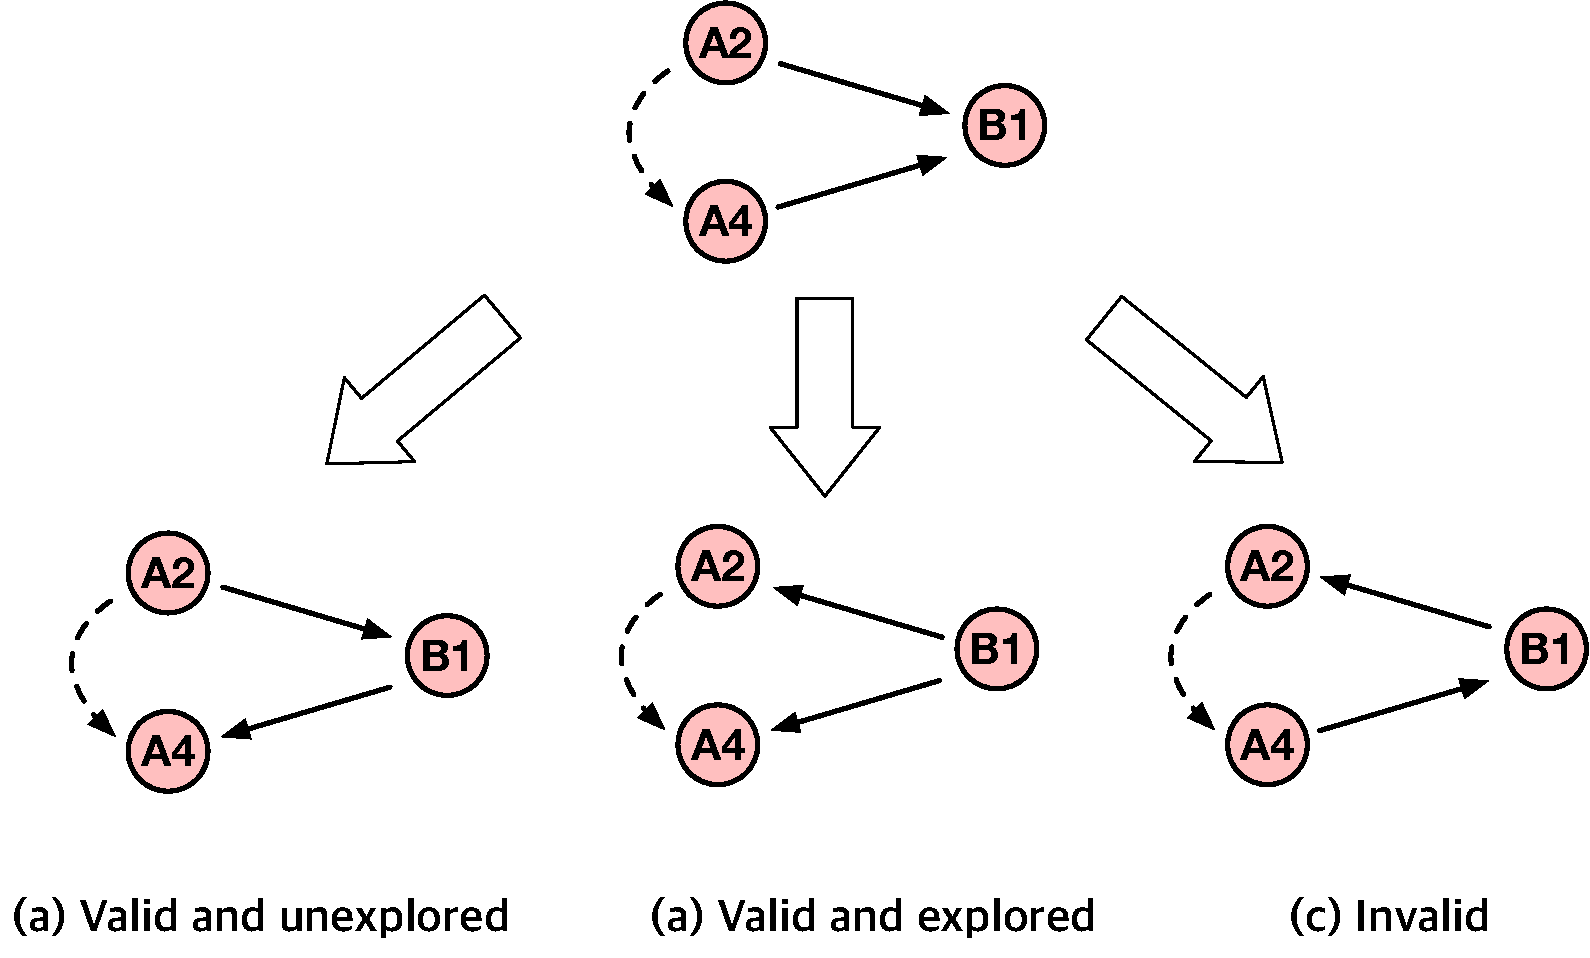
\includegraphics[width=0.9\linewidth]{fig/interleavingmutation.pdf}
  \caption{Example interleaving segment graphs derived from
    \texttt{Segment \#1}. The fuzzer will explore (a) and (b), but
    will not explore (c) contains a loop.}
  \label{fig:interleavingmutation}
\end{figure}
%

\autoref{fig:interleavingmutation} illustrates three examples of
derived segment graphs.
%
The fuzzer flips $\texttt{A4} \Rightarrow \texttt{B1}$ from a given
\texttt{Segment \#1} to generate another segment graph described in
(a).
%
The semantic behind ``\textit{flipping an interleaving edge}'' is
simple; it changes the interleaving order of an instruction pair that
access the shared data.
%
With the segmant graph of (a), the fuzzer will explore thread
interleaving that
$(\texttt{A2} \Rightarrow \texttt{B1}) \wedge (\texttt{B1} \Rightarrow
\texttt{A4})$ (\ie, the condition to cause the uninitialized access
bug).
%
Likewise, the fuzzer generates a segment graph of (b) by flipping both
of $\texttt{A2} \Rightarrow \texttt{B1}$ and
$\texttt{A4} \Rightarrow \texttt{B1}$.
%
Besides (a) and (b), flipping $\texttt{A2} \Rightarrow \texttt{B1}$
can generate the segment graph described in (c). However, This segment
graph is excluded because it contains a loop; a loop indicates a
contradiction on the execution order that any vertex on the loop
should be executed before itself.


It is worth noting that we do not flip program-order edges (\ie,
dotted arrows) with an assumption that thread interleaving do not
change the execution order of instructions executed by a single
thread.
%
In other words, our approach changes thread interleaving while
preserving the order in which instructions occur in the source code.



% Then, the fuzzer excludes 1) ones thas are explored before, and 2)
% ones that contain a loop.
% %
% The reason why the fuzzer excludes explored interleaving segment
% graphs is intuitive; the fuzzer wants to deprioritize interleaving
% segment graphs already explored (such as the case of (b)).
% %
% The fuzzer also excludes ones that contain a loop because.



As a last step, the fuzzer unions all sets of derived interleaving
segment graphs such that
$S_{derived} = S^{1}_{derived} \cup S^{2}_{derived} \cup ... \cup
S^{n}_{derived}$, and uses $S_{derived}$ later to generate scheduling
points.




\PP{Selecting interleaving segments to direct the fuzzer}
%
As described  \autoref{fig:hint}, multiple segment graphs can be
explored at a time (\ie, one thread interleaving comprises multiple
interleaving segments).
%
Thus, our strategy to to quickly consume $S_{derived}$ (\ie, a set of
derived and unexplored segment graphs) is selecting multiple
interleaving segments from $S_{derived}$, and explore them altogether.


However, not all interleaving segments cannot be explored together.
%
For example, in \autoref{fig:hint}, (a) and (b) cannot be explored
together; the segment graph (a) requires \texttt{A2} to be executed
before \texttt{B1} while the segment graph (b) requires the opposite
execution order between \texttt{A2} and \texttt{B1}.
%
Therefore, the fuzzer repeatedly selects and tests a subset of
$S_{derived}$ that is contradiction-free (\ie, does not make a
contradiction on the execution order) until $S_{derived}$ is empty.


It may require a heavy computation to identify the largest
contradiction-free subset of $S_{derived}$.
%
Instead of finding an optimal solution, we choose to adopt a greedy
heuristic.
%
Specifically, we start with an empty set $\bar{S}$. Then, we iterate
over derived segment graphs contained in given $S_{derived}$, and
determine adding each segment graph into $\bar{S}$ forms a loop or
not. If it does not form a loop, we add the segment graph into
$\bar{S}$.
%
After iterating all derived segment graphs in $S_{derived}$, $\bar{S}$
does not contain a loop. The fuzzer then excludes selected segment
graphs from the set of all derived segment graphs (\ie,
$S_{derived} = S_{derived} \setminus \bar{S}$), and generates
scheduling points to explore $\bar{S}$.









\PP{Generating scheduling points}
%
After selecting interleaving segment graphs, generating scheduling
points can be easily done by conducting a topological
sort~\cite{topologicalsort}.
%
Since an imaginary interleaving graph is acyclic, a topological sort
always returns a sequence of vertices (\ie, instructions) that does
not violate a program order.
%
It is well known that the time complexity of a topological sort is
$O(V+E)$. Considering that the graph is sparse, $E$ is a small value
so the time complexity can be asymptotically considered as $O(V)$.
%
In this sequence, scheduling points are just instructions that the
preemption should happen; \ie, the next instruction is executed by a
different thread.




%%% Local Variables:
%%% mode: latex
%%% TeX-master: "p"
%%% End:
